\chapter{实验与结果分析}

\section{实验环境与配置}

\subsection{硬件环境}

% ============================================================
% 【示例：三线表（使用 booktabs 宏包）】
% ============================================================
\begin{table}[htbp]
  \centering
  \caption{实验硬件环境配置}
  \label{tab:hardware}
  \begin{tabular}{ll}
    \toprule
    \textbf{配置项} & \textbf{参数} \\
    \midrule
    CPU         & Intel Core i9-13900K \\  % TODO: 改成你实际的配置
    GPU         & NVIDIA RTX 4090 (24GB) \\
    内存        & 64 GB DDR5 \\
    操作系统    & Ubuntu 22.04 LTS \\
    \bottomrule
  \end{tabular}
\end{table}

\subsection{软件环境}

\begin{table}[htbp]
  \centering
  \caption{实验软件环境配置}
  \label{tab:software}
  \begin{tabular}{ll}
    \toprule
    \textbf{软件/库} & \textbf{版本} \\
    \midrule
    Python       & 3.10 \\  % TODO: 改成你实际的版本
    PyTorch      & 2.1.0 \\
    CUDA         & 12.1 \\
    FFmpeg       & 6.0 \\
    NVIDIA Video Codec SDK & 12.0 \\
    ElegantRL\cite{ref26-liu2021elegantrl} & -- \\
    \bottomrule
  \end{tabular}
\end{table}

\subsection{数据集}

实验使用UVG数据集\cite{ref28-mercat2020uvg}中的1080p分辨率、YUV420格式（NV12转换）视频序列进行测试，序列时长至少为3秒。

\begin{table}[htbp]
  \centering
  \caption{测试视频序列}
  \label{tab:sequences}
  \begin{tabular}{lccl}
    \toprule
    \textbf{序列名称} & \textbf{分辨率} & \textbf{帧率} & \textbf{内容描述} \\
    \midrule
    BasketballDrive  & $1920 \times 1080$ & 50fps  & 运动场景（篮球） \\
    ParkScene        & $1920 \times 1080$ & 24fps  & 自然风景（公园） \\
    Kimono1          & $1920 \times 1080$ & 24fps  & 人物动作（和服） \\
    Cactus           & $1920 \times 1080$ & 50fps  & 复杂纹理（仙人掌） \\
    BQTerrace        & $1920 \times 1080$ & 60fps  & 城市场景（广场） \\
    \bottomrule
  \end{tabular}
\end{table}


\section{评价指标}

本文采用以下指标对实验结果进行评价：

\begin{itemize}
  \item \textbf{BD-Rate (Bjøntegaard Delta Rate)}：衡量两条率失真曲线之间码率节省百分比，负值表示节省码率；
  \item \textbf{LPIPS (Learned Perceptual Image Patch Similarity)}：基于深度学习的感知质量评价指标，值越低越好；
  \item \textbf{SSIM (Structural Similarity Index)}：结构相似性指标，范围$[0, 1]$，越高越好；
  \item \textbf{PSNR (Peak Signal-to-Noise Ratio)}：峰值信噪比，单位dB，越高越好；
  \item \textbf{模型参数量}：衡量模型复杂度，单位为K/M参数个数；
  \item \textbf{推理时间}：单帧推理耗时，衡量实时性。
\end{itemize}


\subsection{BD-LPIPS分析}

实验结果表明，基于强化学习的RAPNet前处理框架在LPIPS感知质量指标上相比Baseline取得了显著的BD-LPIPS优化。各视频序列的详细测试结果如表~\ref{tab:bdlpips-results}所示。

\begin{table}[htbp]
  \centering
  \caption{RAPNet前处理框架测试结果}
  \label{tab:bdlpips-results}
  \begin{tabular}{lcccc}
    \toprule
    \textbf{视频序列} & \textbf{Baseline平均LPIPS} & \textbf{$\Delta$LPIPS(\%)} & \textbf{$\Delta$码率(\%)} & \textbf{BD-LPIPS(\%)} \\
    \midrule
    BasketballDrive  & 0.4664 & $-11.53$ & $+1.02$  & $\mathbf{-12.84}$ \\
    ParkScene        & 0.5313 & $-4.51$  & $-11.08$ & $\mathbf{-13.45}$ \\
    Kimono1          & 0.4513 & $-1.78$  & $+3.74$  & $\mathbf{-5.62}$  \\
    Cactus           & 0.4349 & $+1.92$  & $-13.62$ & $\mathbf{-11.15}$ \\
    BQTerrace        & 0.4250 & $+0.54$  & $-4.95$  & $\mathbf{-4.32}$  \\
    \midrule
    \textbf{平均(Average)} & \textbf{0.4618} & $\mathbf{-3.07}$ & $\mathbf{-4.98}$ & $\mathbf{-9.48}$ \\
    \bottomrule
  \end{tabular}
\end{table}

从表~\ref{tab:bdlpips-results}可以看出，RAPNet在所有测试序列上均取得了负的BD-LPIPS值，平均BD-LPIPS为$-9.48\%$，表明在相同感知质量下可节省约9.48\%的码率。其中，ParkScene和BasketballDrive序列的改善最为显著，BD-LPIPS分别达到$-13.45\%$和$-12.84\%$。值得注意的是，Cactus序列虽然LPIPS略有上升($+1.92\%$)，但码率大幅下降($-13.62\%$)，综合BD-LPIPS仍达到$-11.15\%$。

图~\ref{fig:rd-curve-results}展示了Baseline与RAPNet在所有测试序列上的平均RD曲线对比。可以看到，RAPNet的RD曲线在所有码率点上均低于Baseline，表明在相同码率下RAPNet能够提供更低的LPIPS（即更好的感知质量）。

\begin{figure}[htbp]
  \centering
  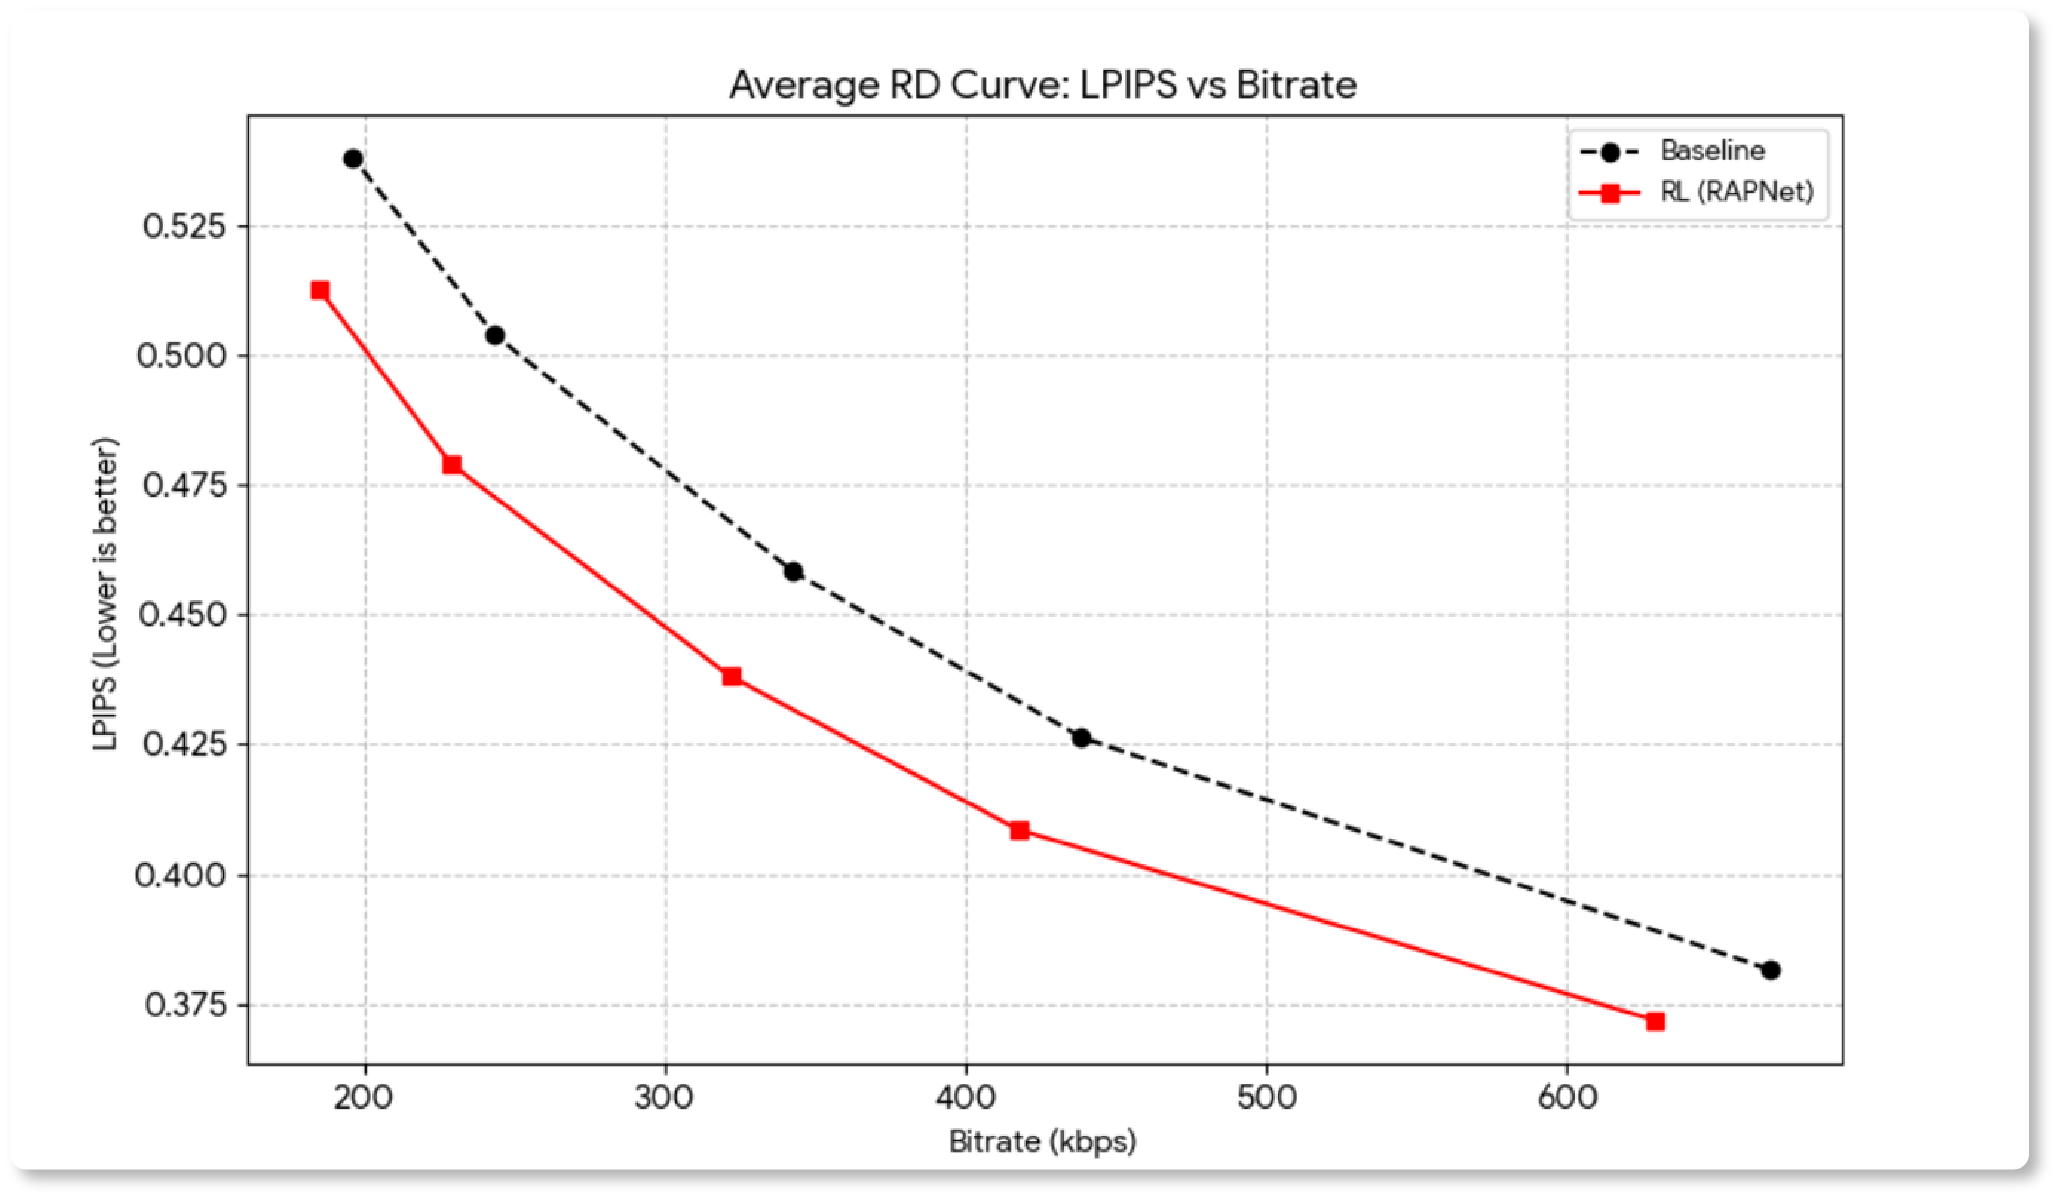
\includegraphics[width=0.75\textwidth]{data/图片测试结果RD曲线.png}
  \caption{Baseline与RAPNet平均RD曲线对比（LPIPS vs 码率）}
  \label{fig:rd-curve-results}
\end{figure}

\subsection{训练过程分析}

图~\ref{fig:training-curves}展示了训练过程中的关键监控指标。从TensorBoard训练曲线可以观察到：（1）delta\_r\_mean（码率节省）在训练前期波动较大，但整体呈正值趋势，表明模型学会了节省码率；（2）delta\_v\_mean（质量提升）在后半段训练中逐渐转正，表明感知质量得到改善；（3）force\_q\_thrust（Critic推力）和force\_mse\_drag（MSE阻力）的动态平衡反映了Actor-Critic架构中``探索与利用''的权衡过程。

\begin{figure}[htbp]
  \centering
  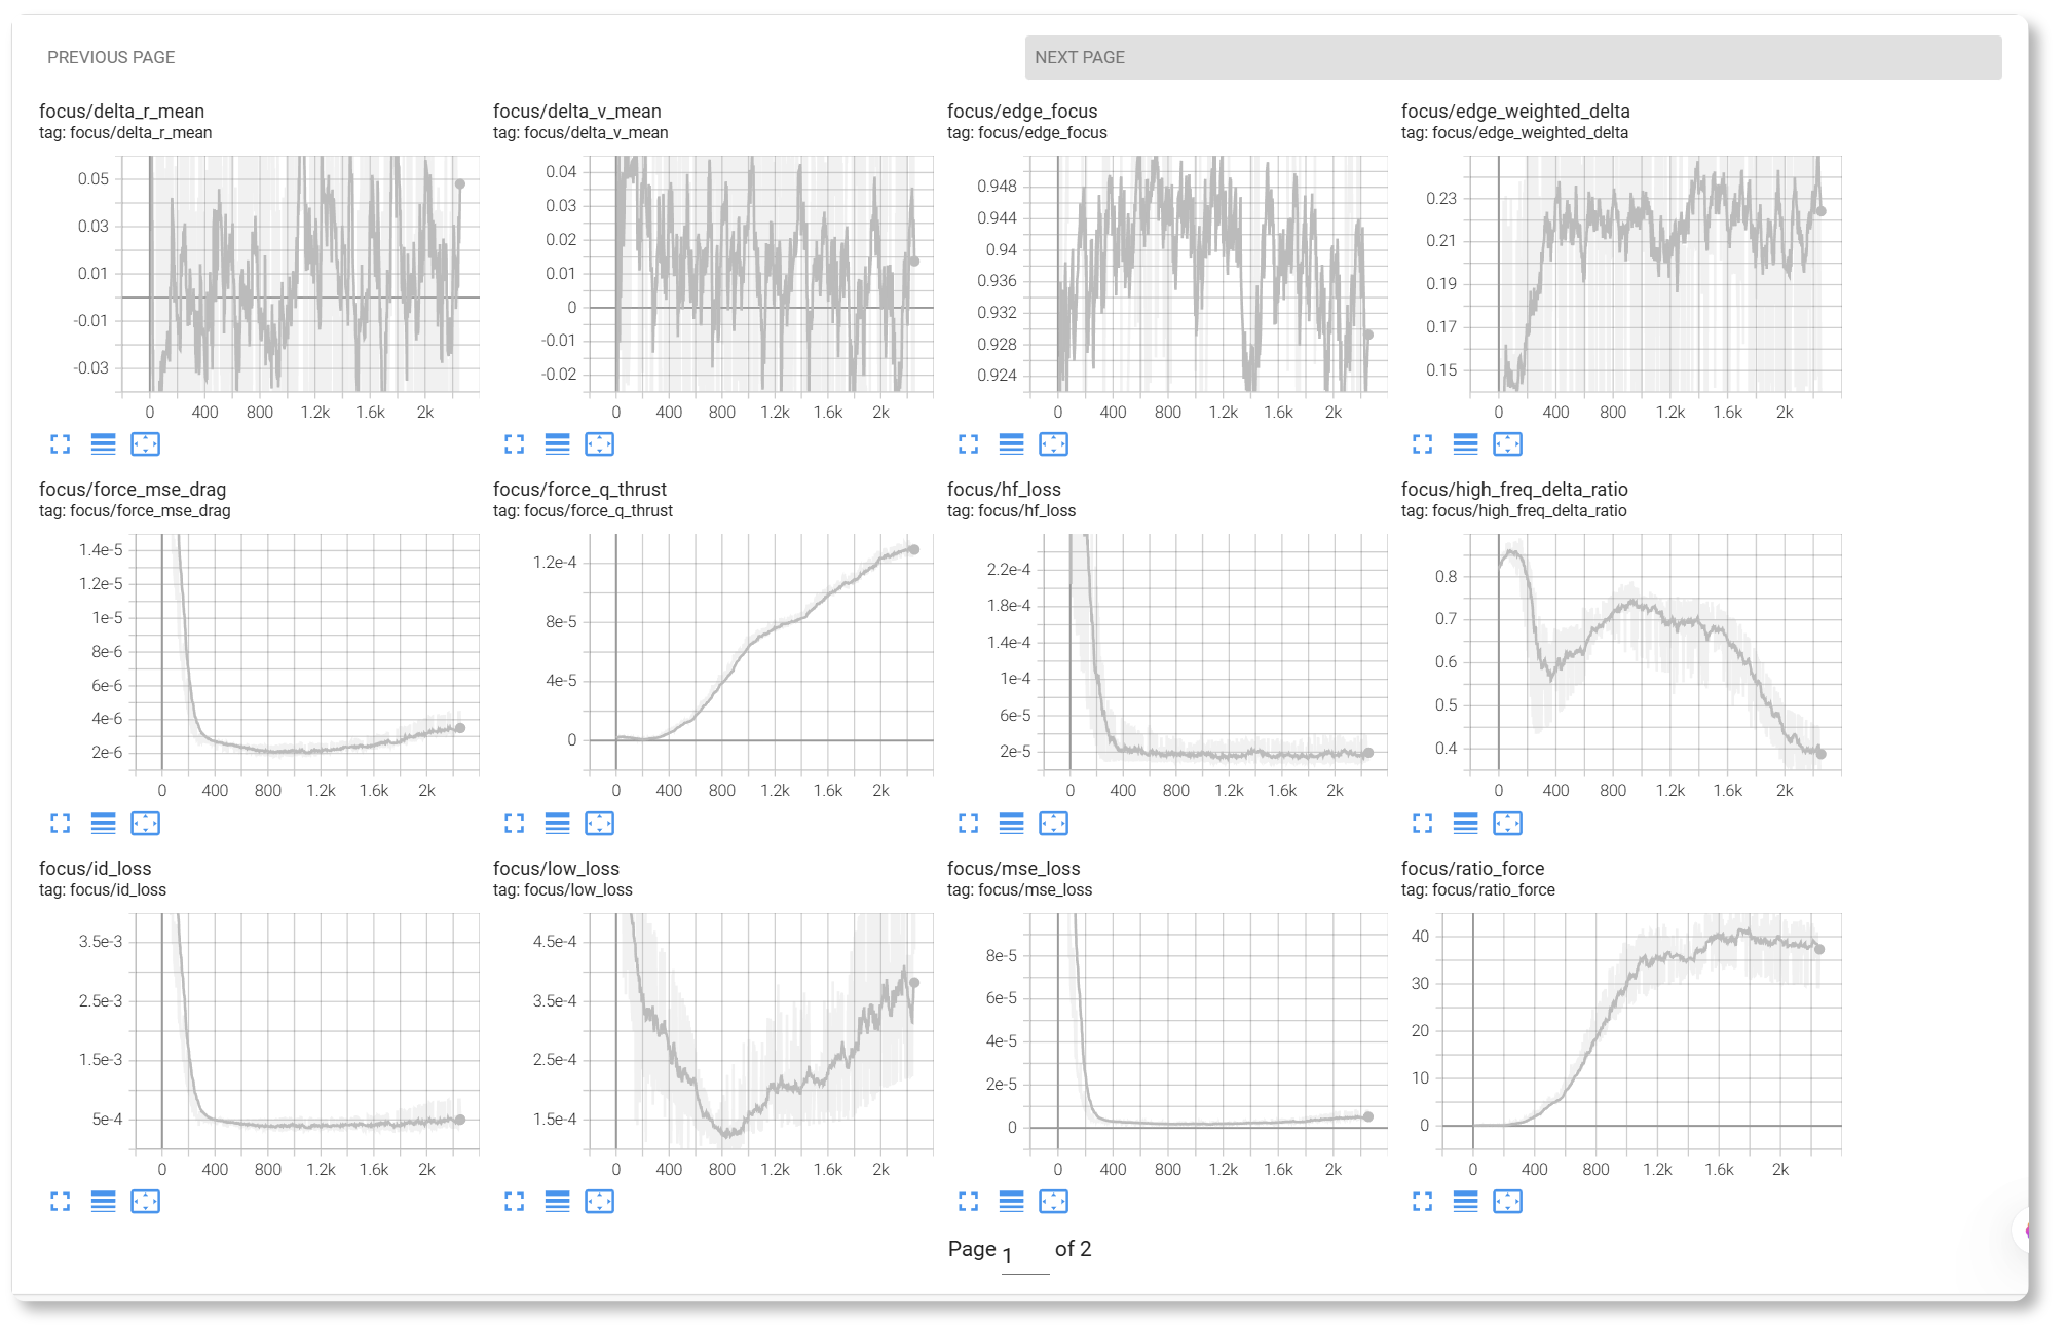
\includegraphics[width=0.95\textwidth]{data/图片训练曲线.png}
  \caption{TensorBoard训练监控曲线}
  \label{fig:training-curves}
\end{figure}

\subsection{频域分析}

图~\ref{fig:freq-training}展示了训练过程中图片频域的变化，可以观察到模型逐渐学会在特定频率方向上进行有针对性的修改。

\begin{figure}[htbp]
  \centering
  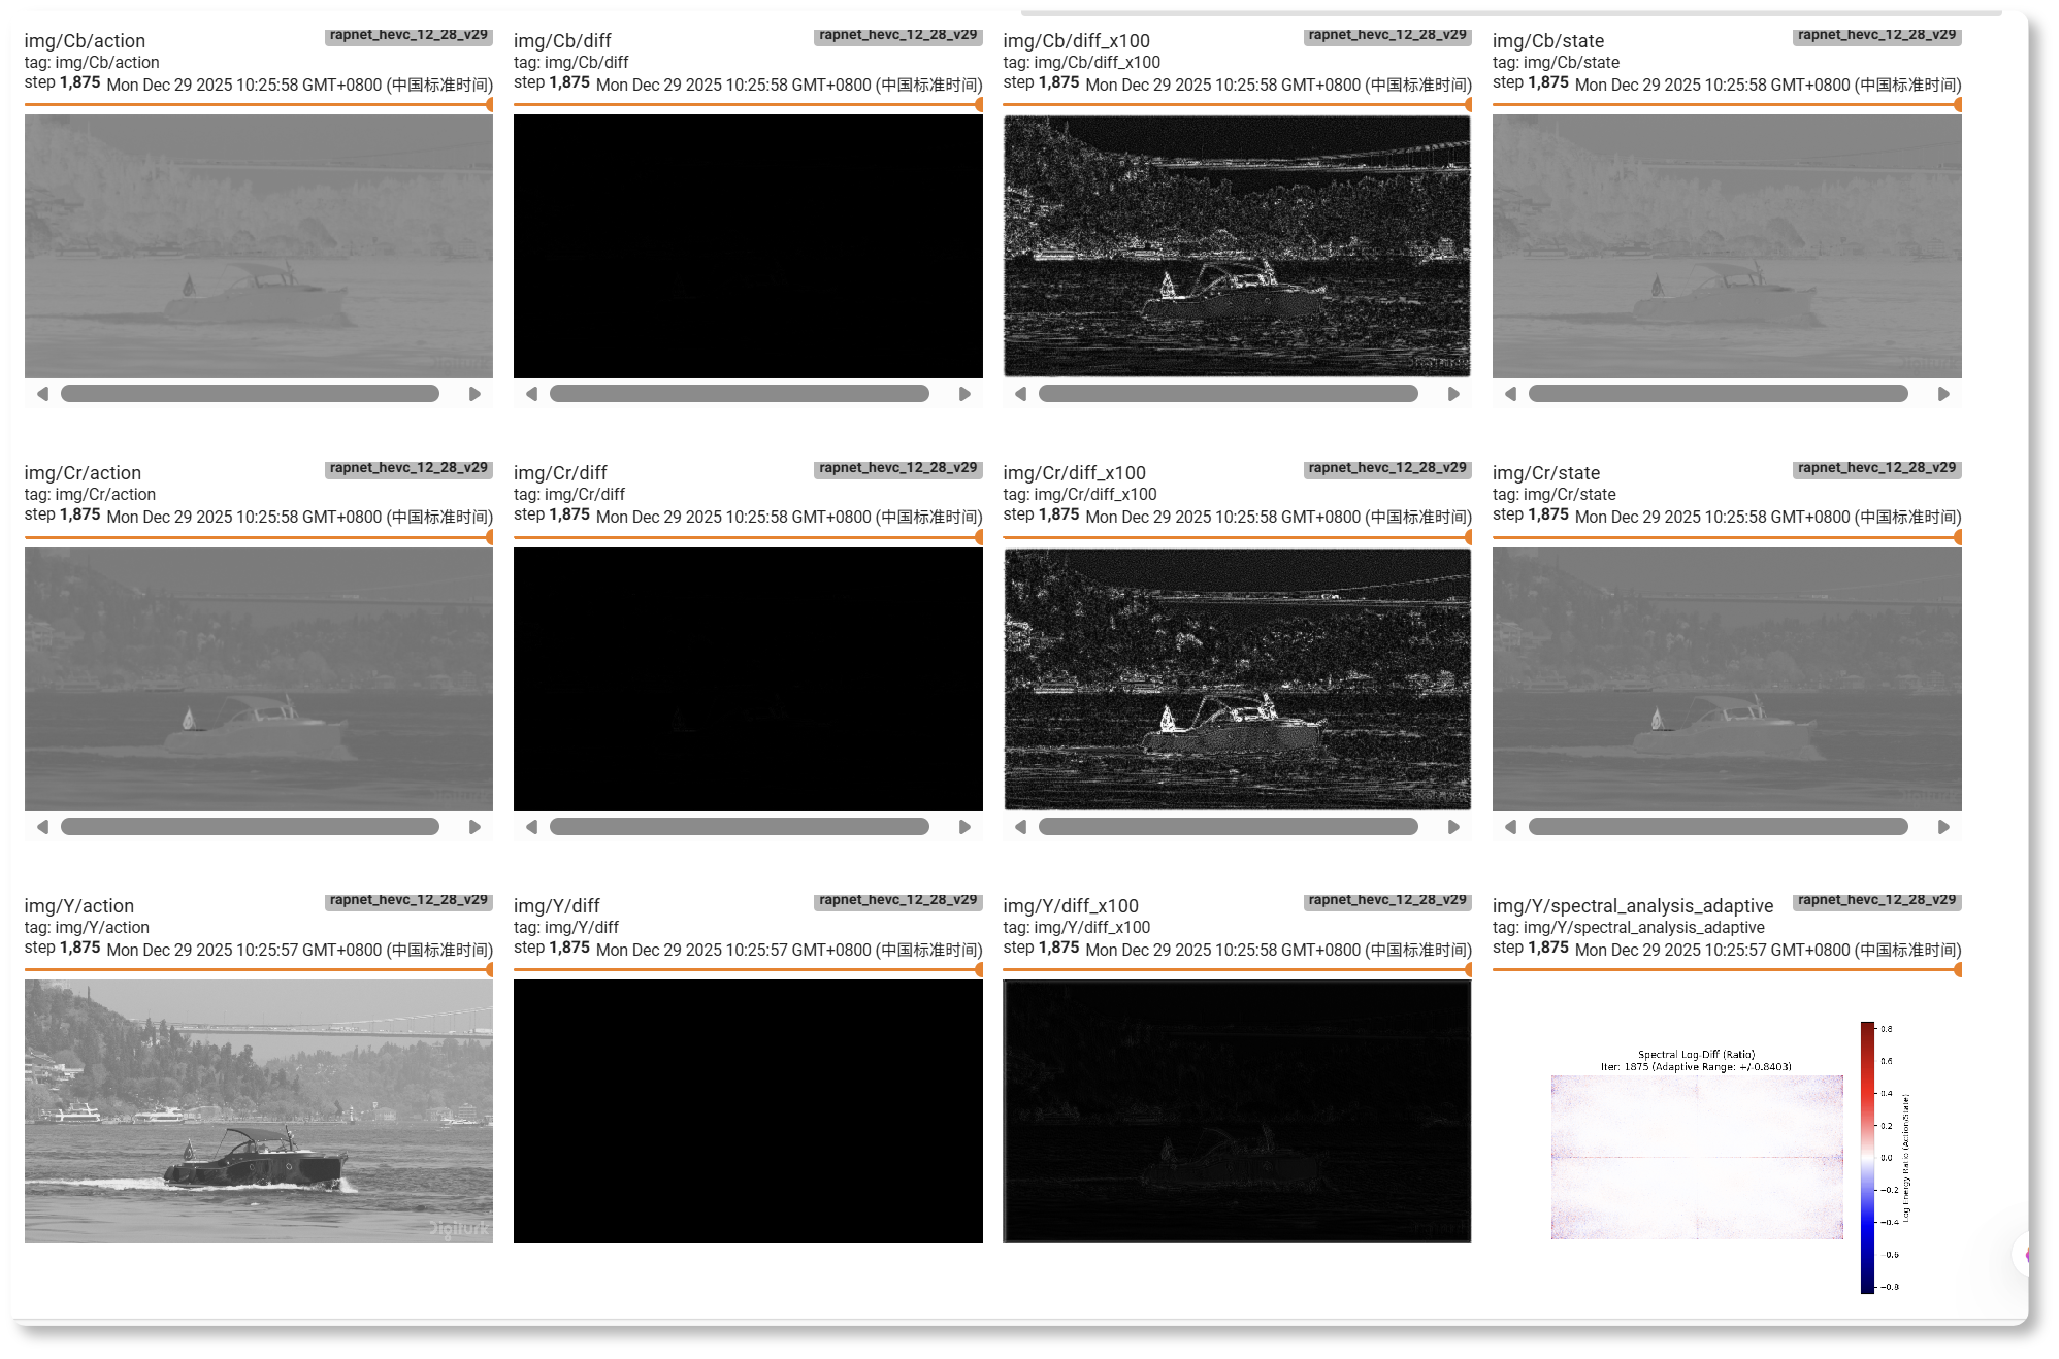
\includegraphics[width=0.95\textwidth]{data/图片训练过程中图片频域变化显示.png}
  \caption{训练过程中图片频域变化}
  \label{fig:freq-training}
\end{figure}

图~\ref{fig:spectrum-analysis}展示了经过充分训练后，模型处理前后图片的频谱差异图（Spectral Log-Diff）。可以看到图片经过模型处理后，主要有如下变化：频谱图在中心及四条边的中点位置出现有规律的红色增强，而四角区域几乎没有明显变化，说明网络主要保留了水平与垂直方向上的主结构分量，未显著增强斜向纹理。这种方向性增强更贴合自然图像的结构特征，同时也使得压缩后的内容在编码器的预测建模中更具可预测性，从而有助于整体编码效率的提升。

\begin{figure}[htbp]
  \centering
  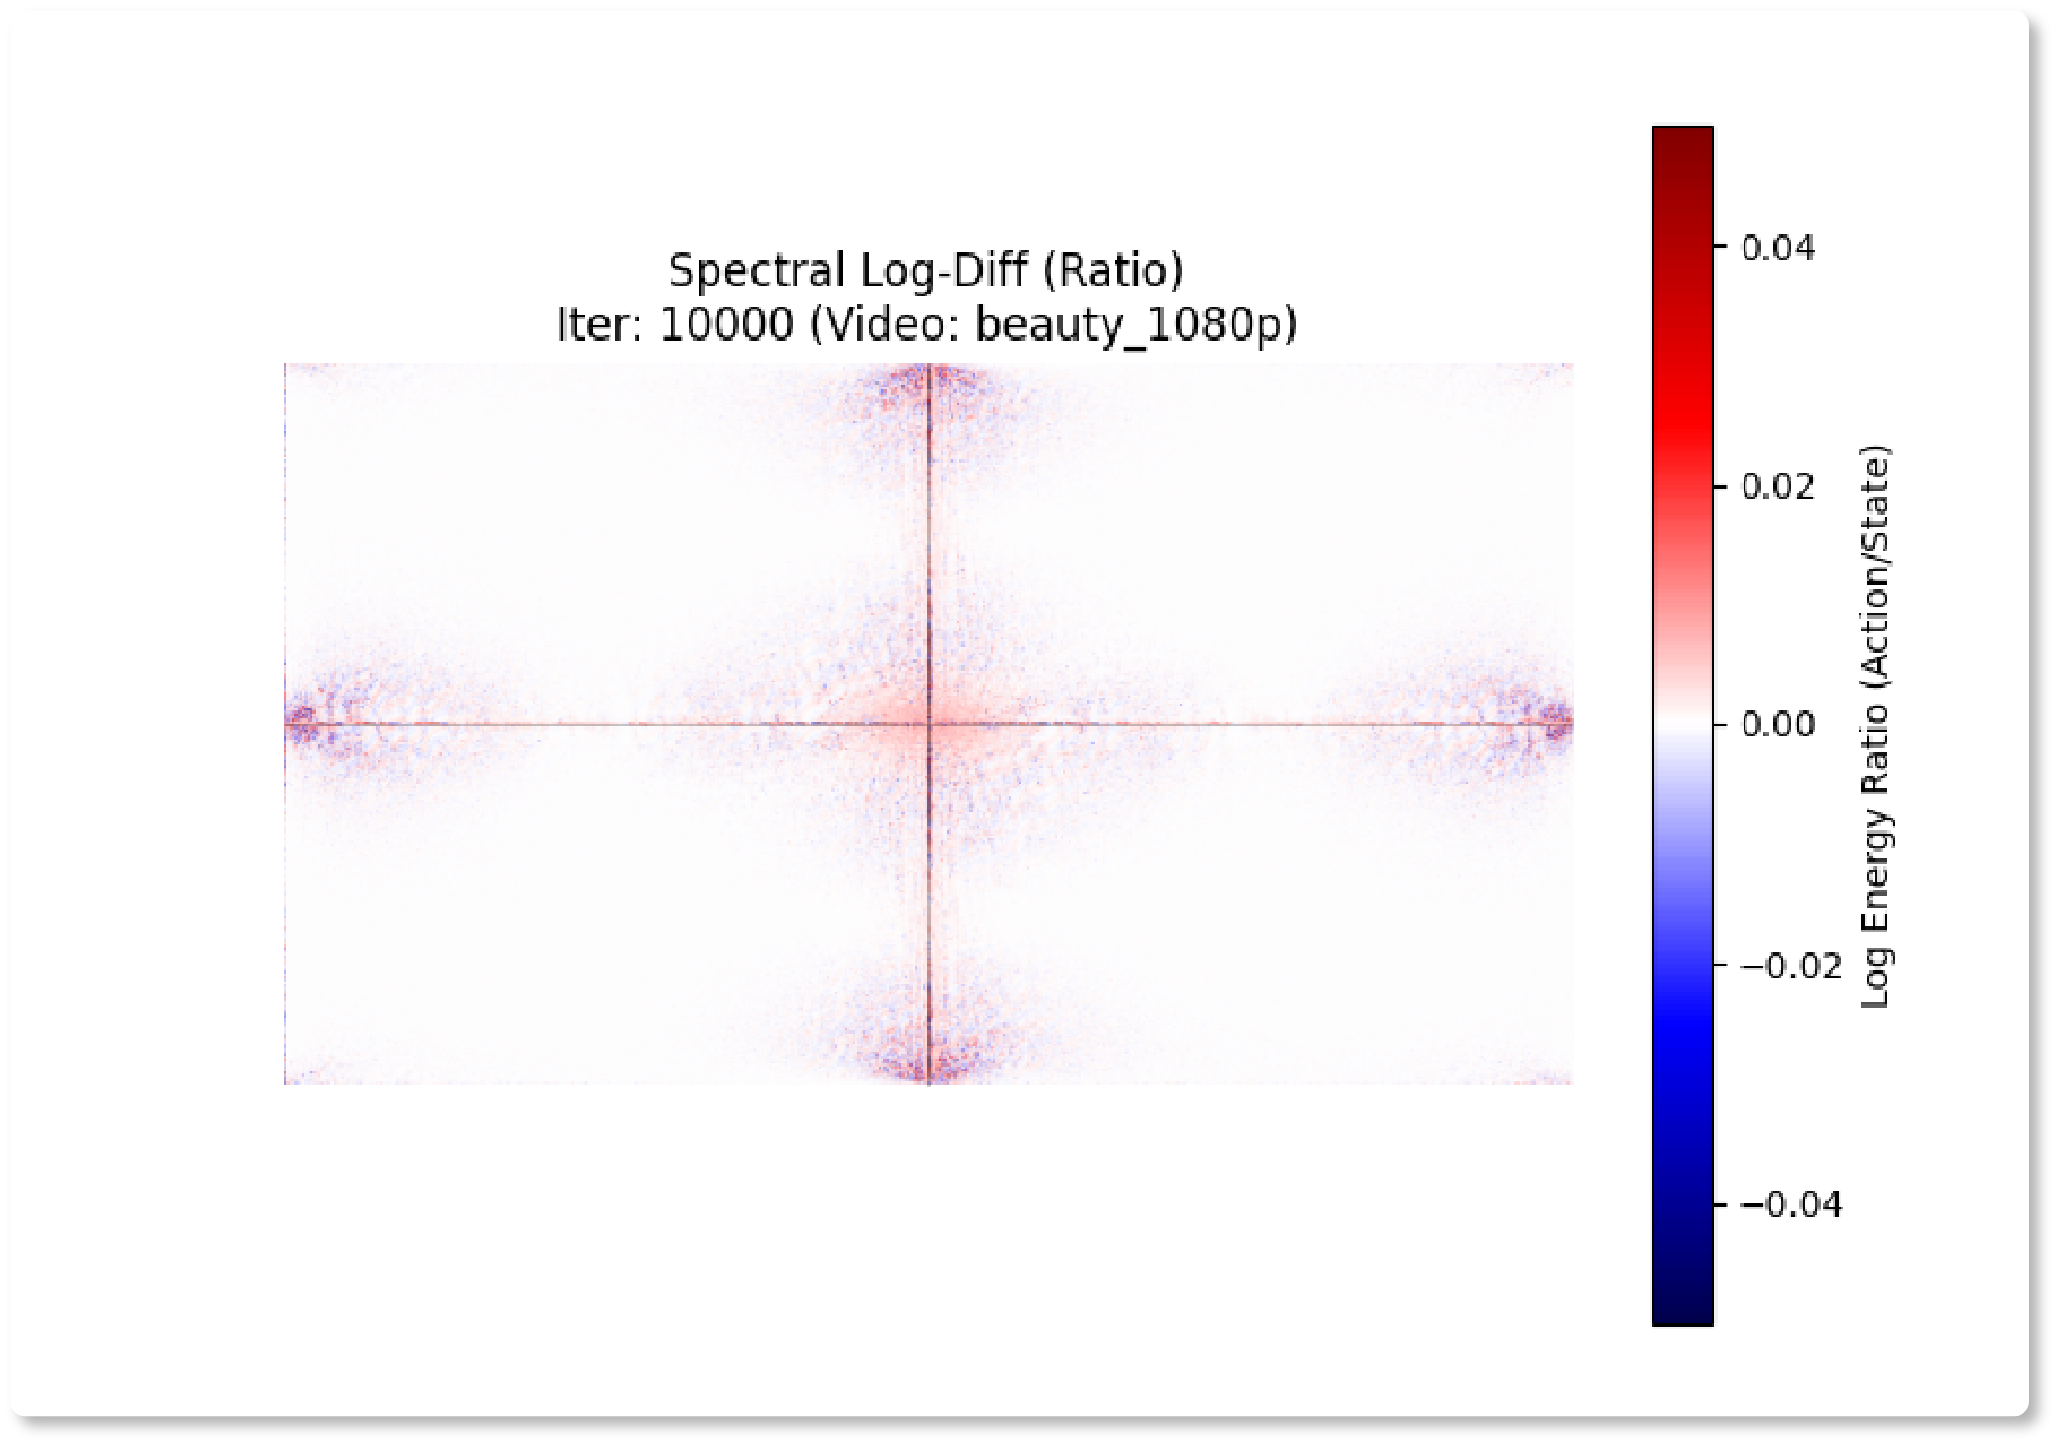
\includegraphics[width=0.75\textwidth]{data/图片模型处理后频谱图.png}
  \caption{模型处理前后频谱差异图（Spectral Log-Diff）}
  \label{fig:spectrum-analysis}
\end{figure}

\subsection{主观视觉效果分析}

% TODO: 插入主观质量对比图（Baseline vs RAPNet 的解码帧截图）


\section{消融实验}

为了验证系统设计中各关键参数的合理性，本节从编码参数选择和损失函数设计两个维度进行了系统性的消融实验。

\subsection{编码参数选择实验}

在正式训练强化学习模型之前，需要确定NVENC硬件编码器的最优参数配置。这些参数直接影响Baseline的率失真性能和训练环境的行为，因此需要通过迭代式实验来确定。

\subsubsection{NVENC Preset选择}

NVENC编码器提供p1至p7共7个编码预设，p1为最快速（最低质量），p7为最慢速（最高质量）。实验对p1至p4四个常用preset进行了编码质量与码率关系的对比分析，结果如图~\ref{fig:preset-compare}所示。

\begin{figure}[htbp]
  \centering
  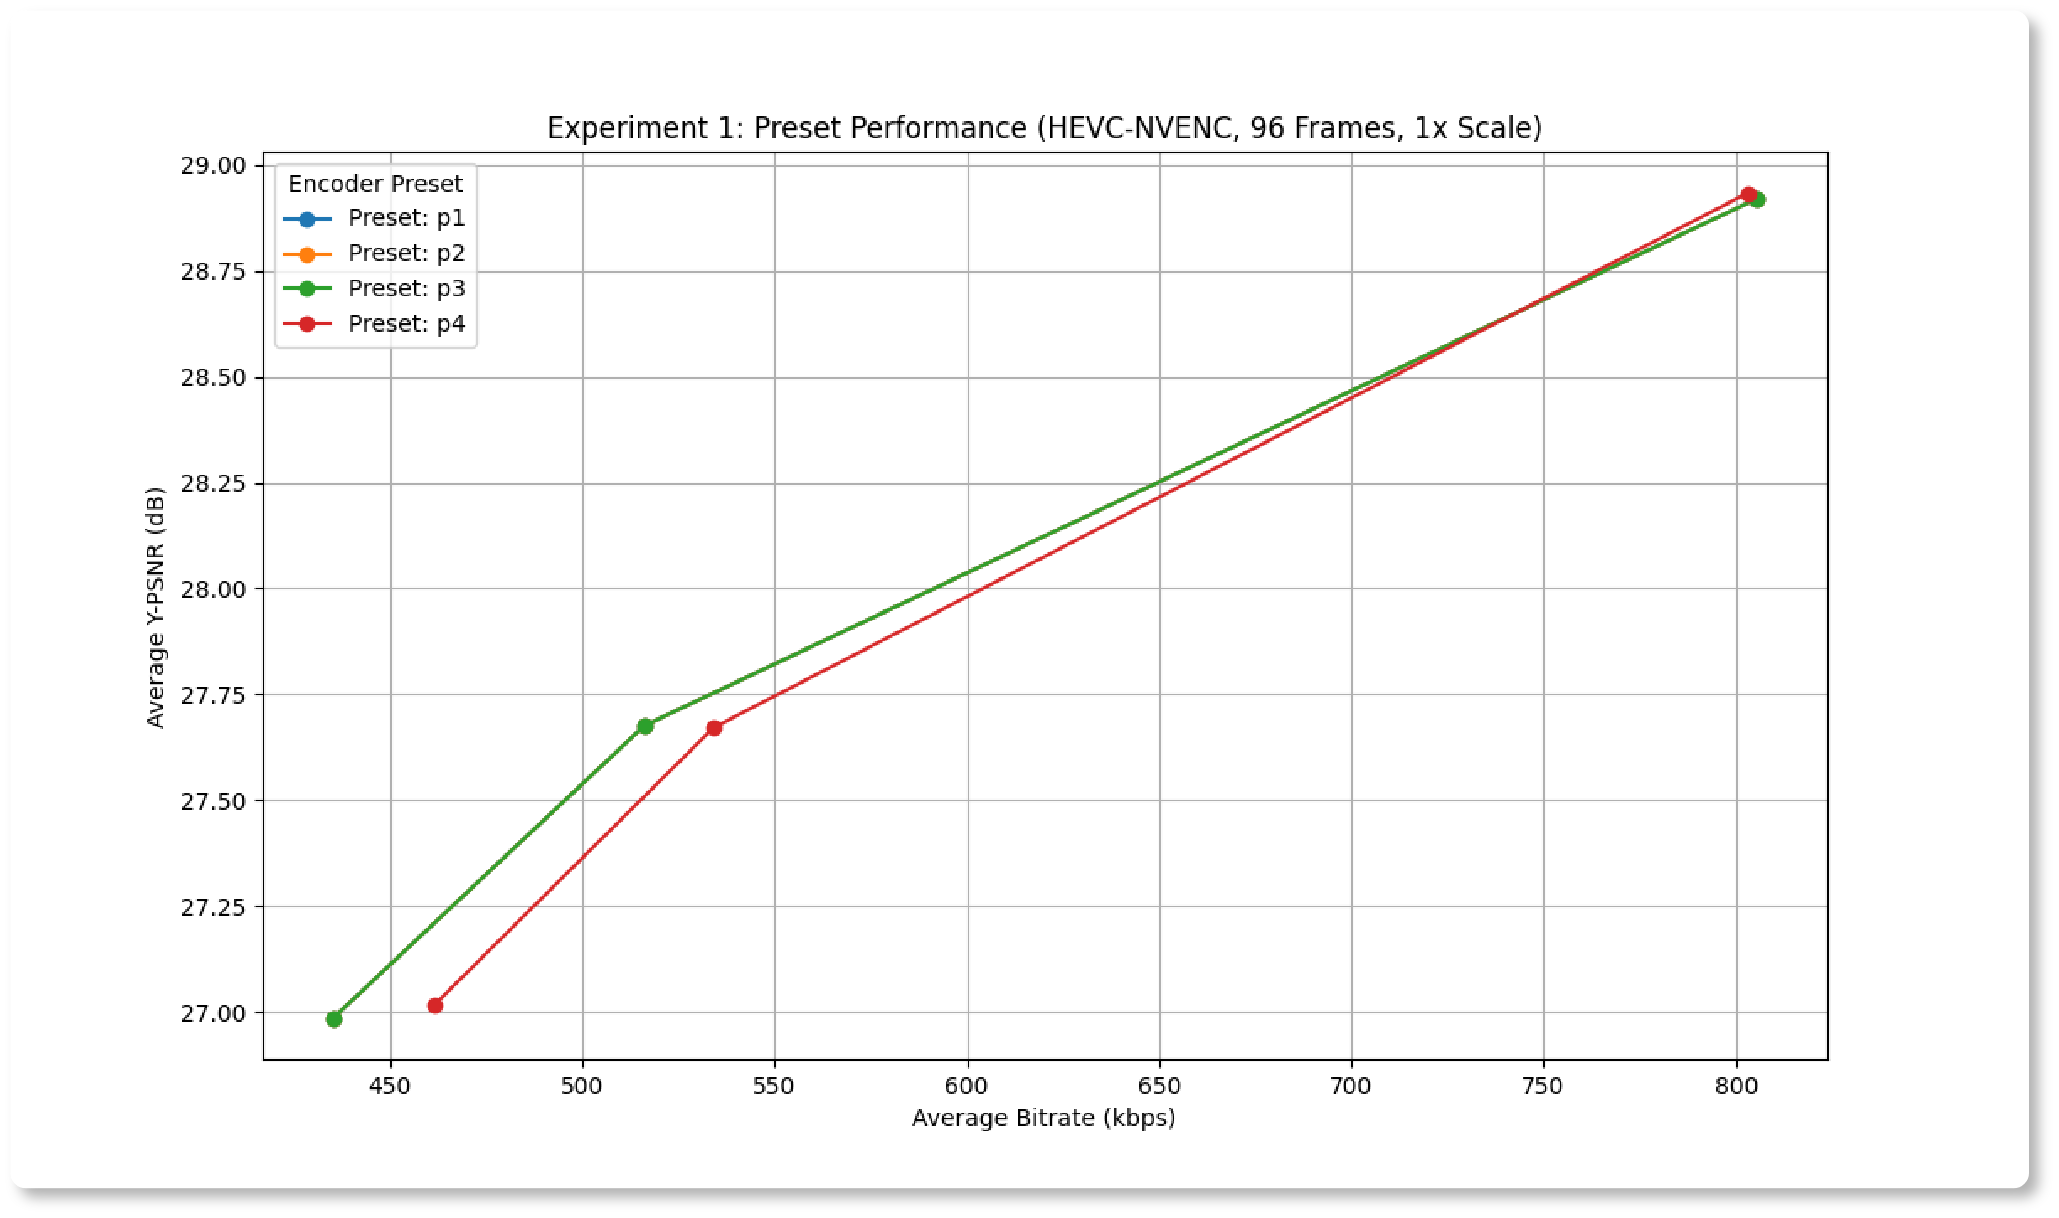
\includegraphics[width=0.8\textwidth]{data/图片Preset对比实验.png}
  \caption{NVENC编码预设对比实验（HEVC-NVENC, 96帧, 1x Scale）}
  \label{fig:preset-compare}
\end{figure}

从图~\ref{fig:preset-compare}可以看出，p1/p2/p3三个预设的RD曲线几乎完全重合，而p4在低码率点（400-600 kbps）上略低于p1-p3，但在高码率点上差异微乎其微。综合编码质量与训练速度，本文选择\textbf{p4 (medium)}作为训练和评估的统一预设。

GOP (Group of Pictures)定义了两个I帧之间的距离。在本文的训练场景中，每个episode编码16帧短clip，第一帧必须为I帧。图~\ref{fig:gop-compare}展示了GOP=$-1$（默认值）和GOP=32两种配置下，不同下采样算法的RD曲线对比。

\begin{figure}[htbp]
  \centering
  \begin{subfigure}[b]{0.48\textwidth}
    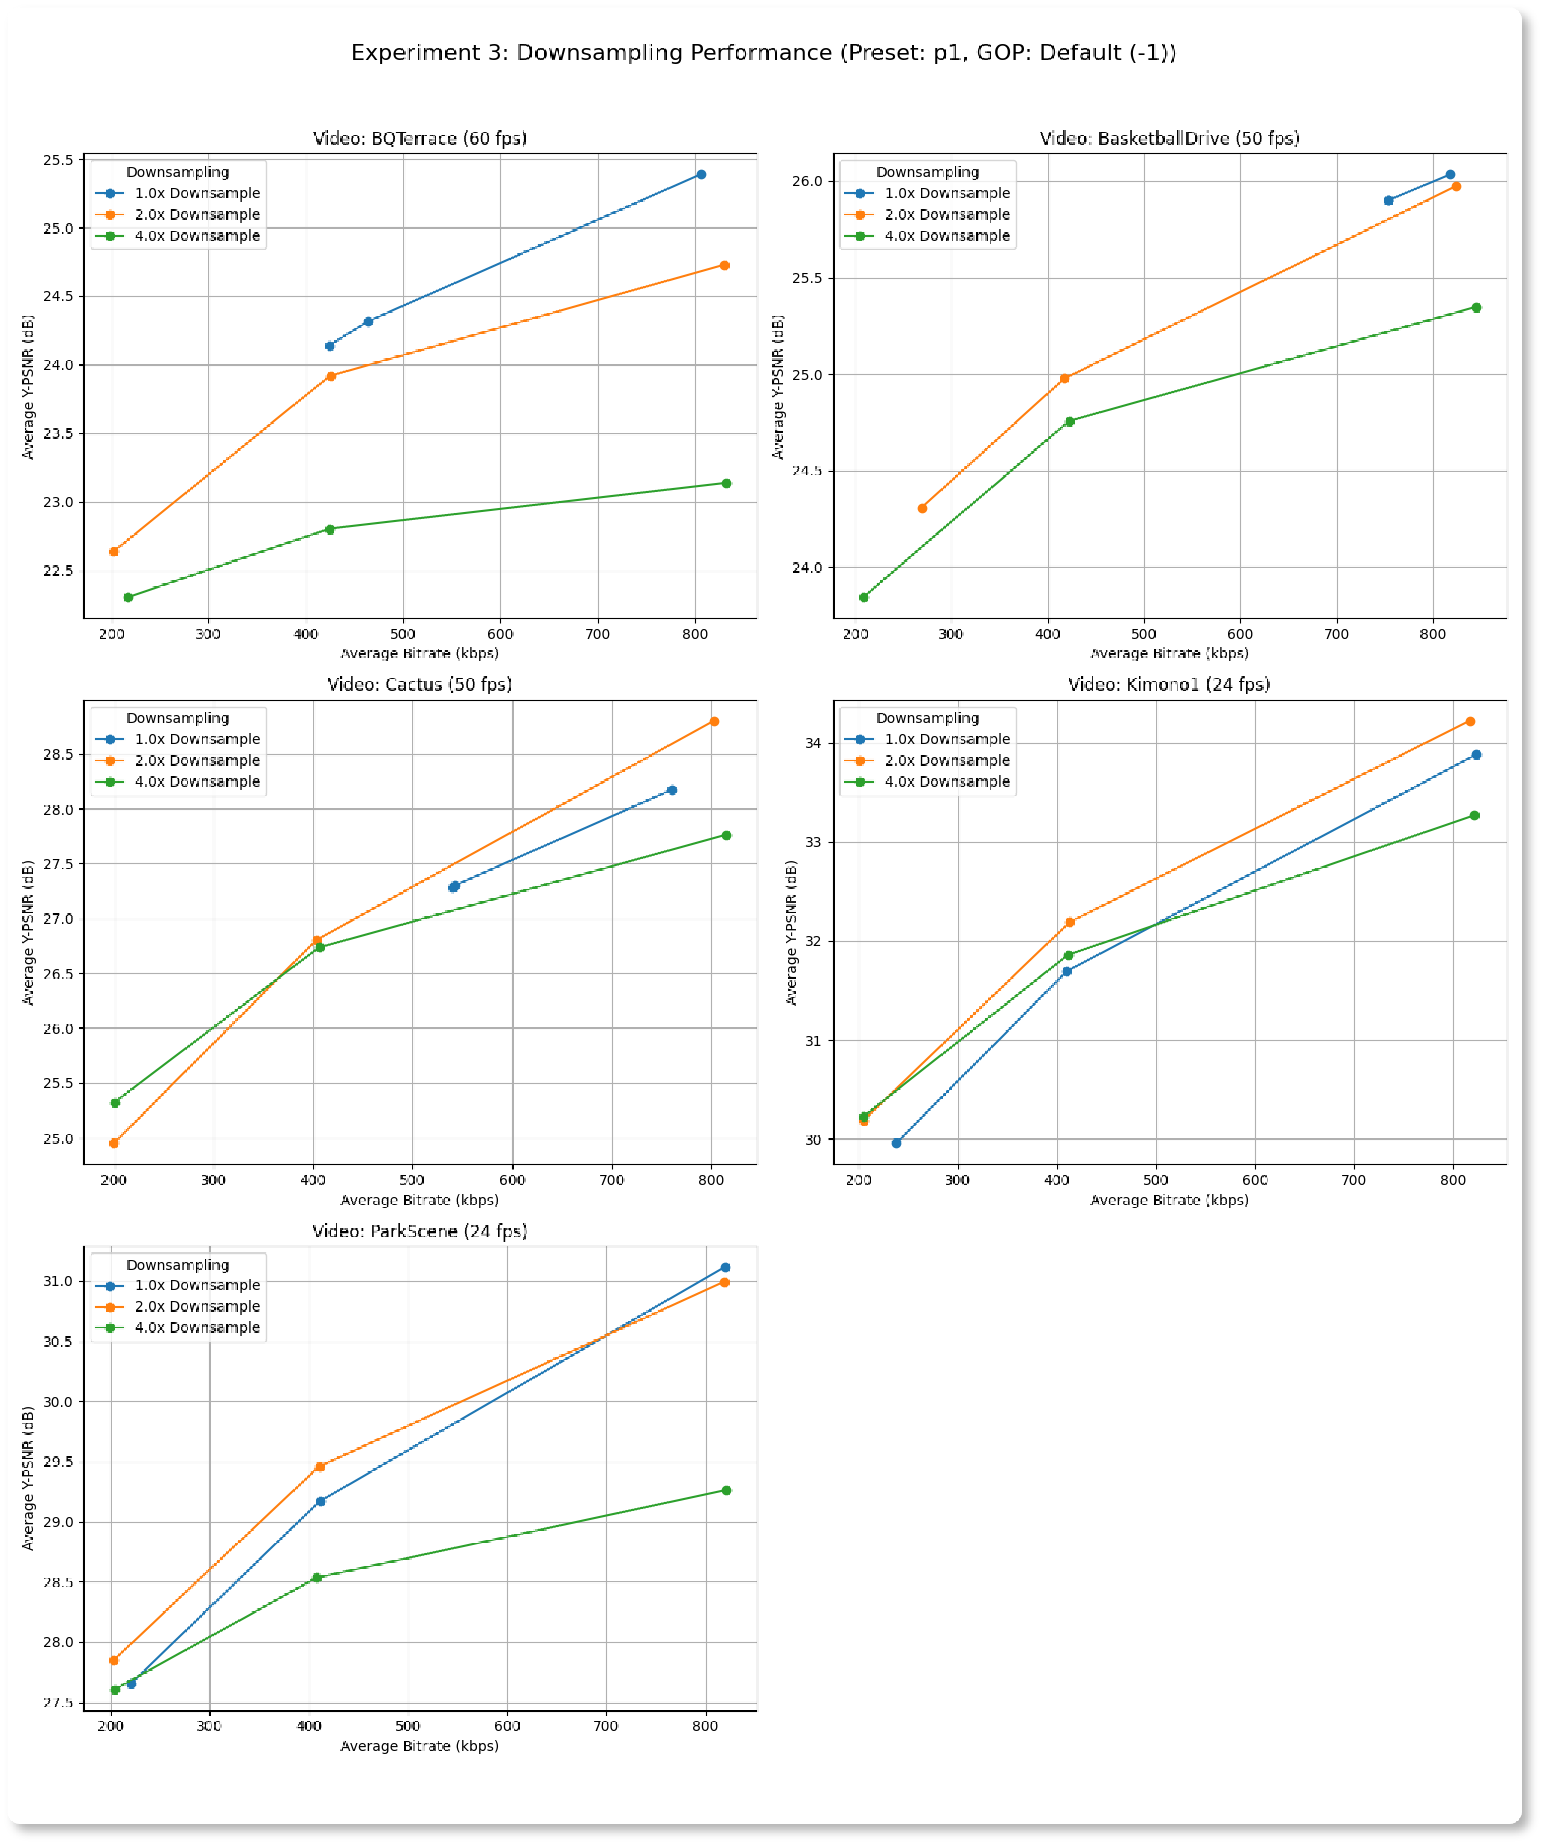
\includegraphics[width=\textwidth]{data/图片GOP = -1.png}
    \caption{GOP=$-1$（默认配置）}
    \label{fig:gop-default}
  \end{subfigure}
  \hfill
  \begin{subfigure}[b]{0.48\textwidth}
    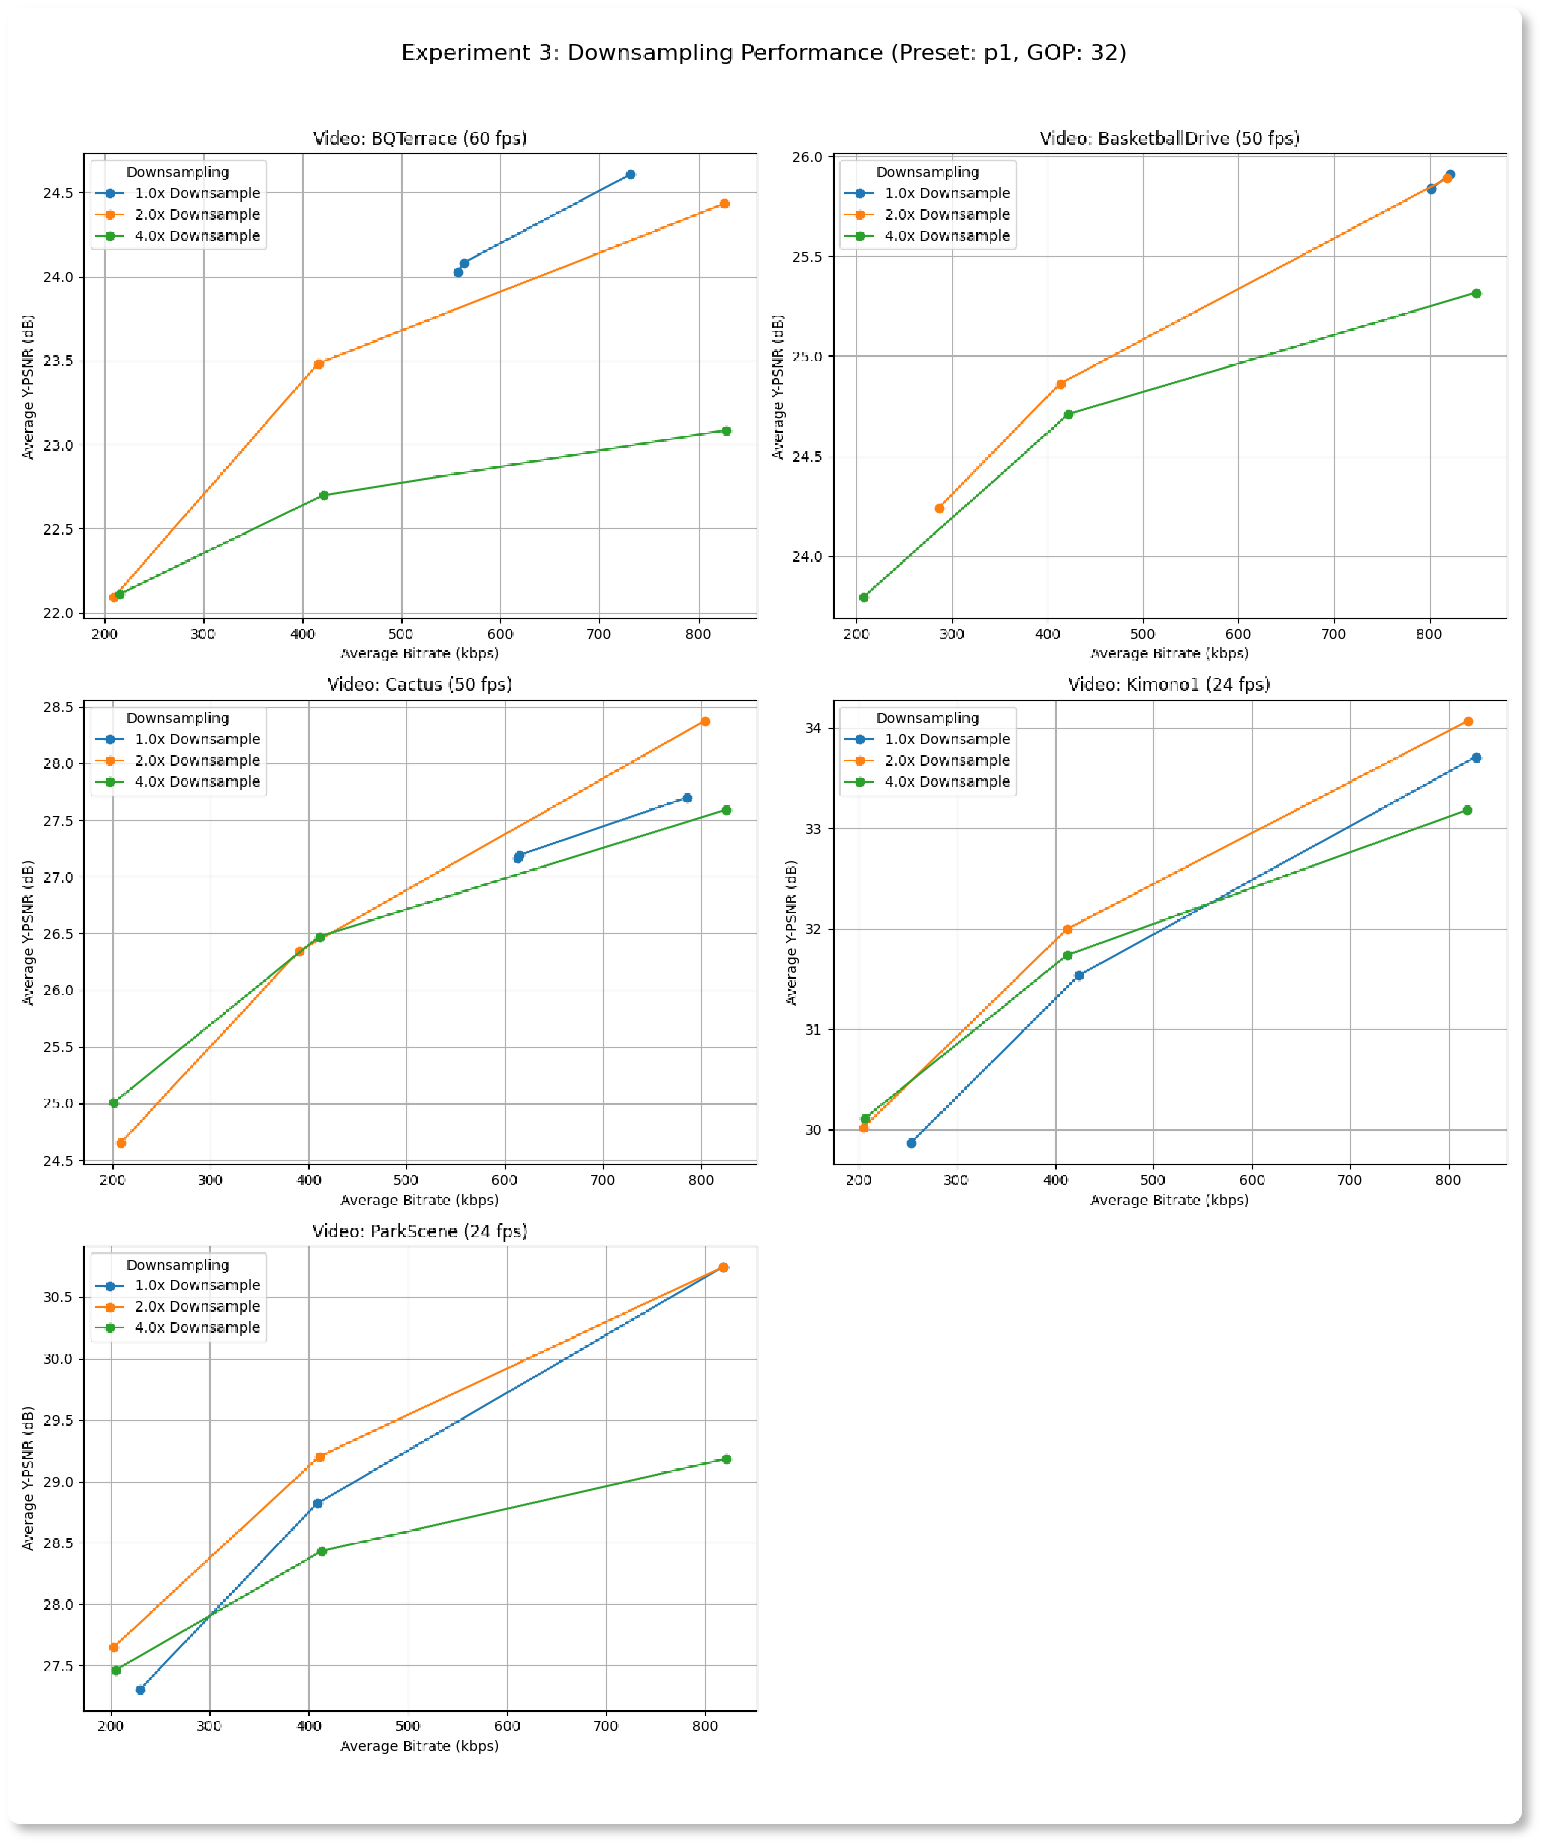
\includegraphics[width=\textwidth]{data/图片GOP=32.png}
    \caption{GOP=32}
    \label{fig:gop-32}
  \end{subfigure}
  \caption{不同GOP配置下的下采样算法RD曲线对比}
  \label{fig:gop-compare}
\end{figure}

从图~\ref{fig:gop-compare}可以观察到，GOP=32配置下各下采样算法的RD曲线整体低于GOP=$-1$配置，这是因为显式设置GOP=32会限制帧间预测的参考距离。经过实验验证，采用\textbf{GOP=$-1$（默认配置）}能够在训练稳定性和编码效率之间取得最佳平衡。

\subsubsection{色彩空间与像素格式}

视频编码标准普遍采用YCbCr色彩空间而非RGB，原因在于：（1）人眼对亮度（Y通道）的敏感度远高于色度（Cb/Cr通道），因此可以对色度进行4:2:0子采样而不显著影响主观质量；（2）Y/Cb/Cr三通道之间的相关性低于R/G/B通道，有利于后续的变换编码。

本系统全程在\textbf{YUV420p}格式下工作：亮度分辨率为$(H, W)$，色度分辨率为$(H/2, W/2)$。训练中需要特别注意：（1）PSNR等客观指标必须在YUV空间计算（Y-PSNR），而非在RGB空间计算，否则会导致结论偏差\footnote{FFmpeg在RGB输入时默认计算R/G/B PSNR，必须通过\texttt{format=yuv420p}强制转换为YUV后再计算。}；（2）随机裁剪坐标必须为2的倍数，以保证YUV420格式下亮度与色度通道的空间对齐。

\subsubsection{下采样算法选择}

在Baseline构建中，需要将1080p视频下采样到540p进行编码。不同的下采样算法对重建质量有显著影响。图~\ref{fig:downsample-compare}展示了5个测试序列在不同下采样倍数（1x/2x/4x）下的Y-PSNR对比。

\begin{figure}[htbp]
  \centering
  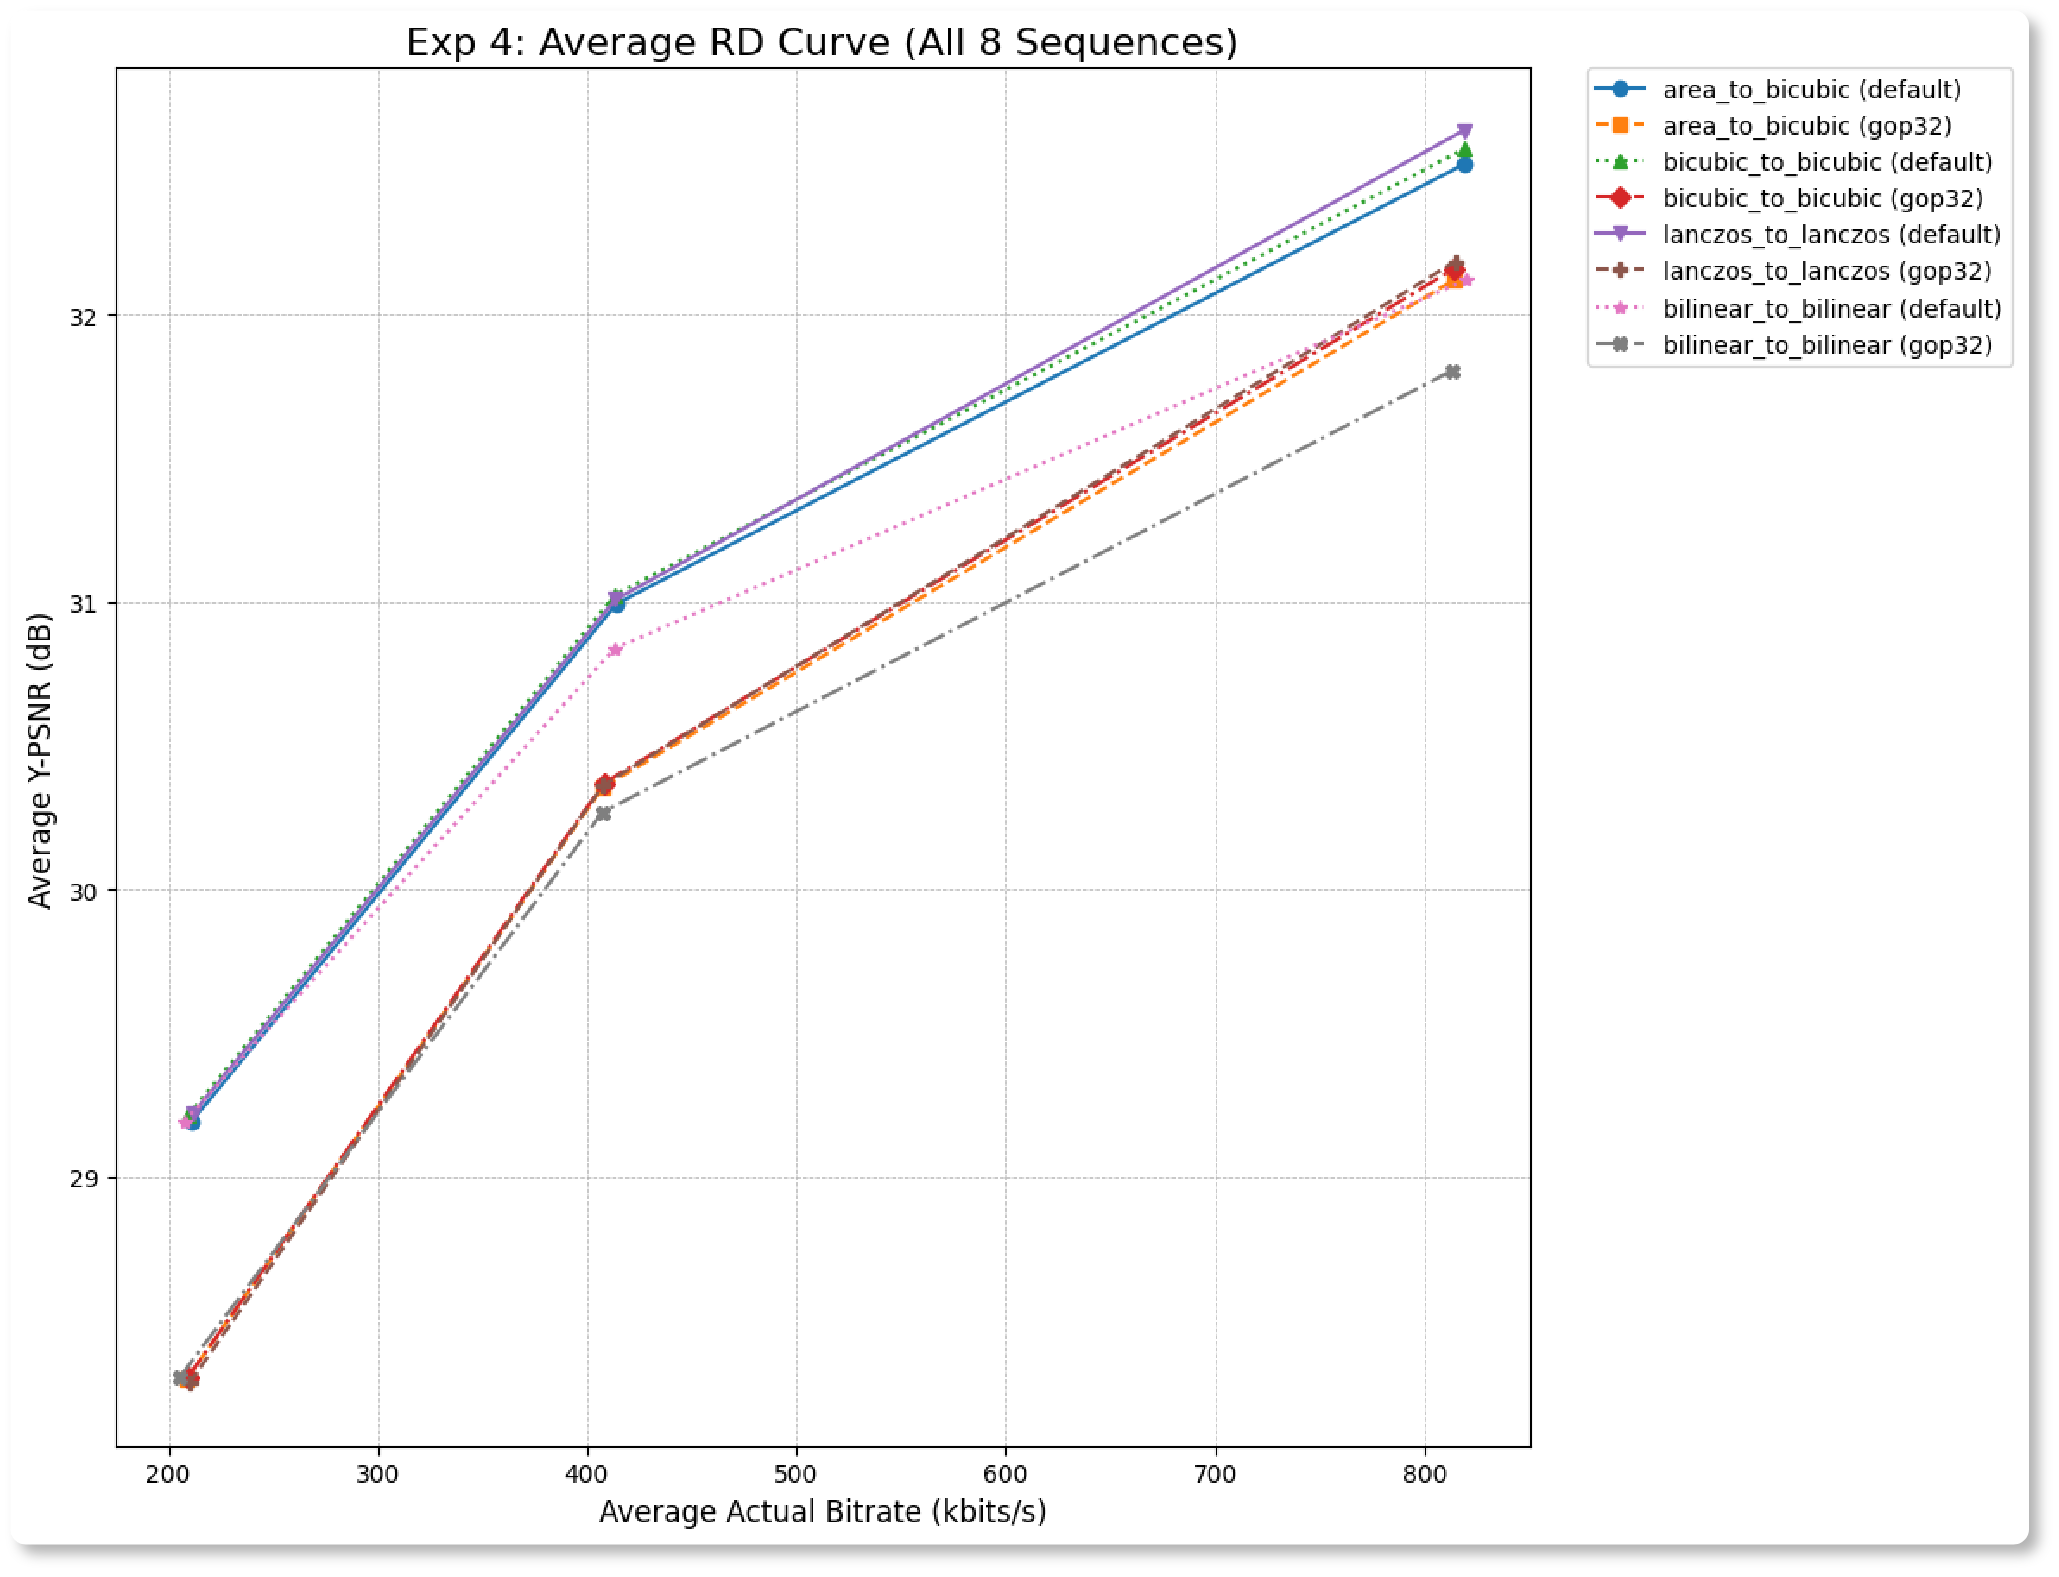
\includegraphics[width=0.85\textwidth]{data/图片下采样算法.png}
  \caption{不同下采样倍数下的Y-PSNR对比（Preset: p1, GOP: Default）}
  \label{fig:downsample-compare}
\end{figure}

从图~\ref{fig:downsample-compare}可以观察到：（1）1x（不下采样）始终提供最优的PSNR，但编码分辨率为原始1080p，码率开销最大；（2）2x下采样在中低码率点上表现良好，是本文采用的编码分辨率；（3）4x下采样导致PSNR显著下降，信息损失过大。结合图~\ref{fig:gop-compare}中的下采样算法对比，Lanczos算法在保持边缘锐度方面具有明显优势，因此本文在需要下采样的场景中统一采用Lanczos算法。

\subsubsection{码率控制模式}

NVENC支持多种码率控制模式，包括CQP（恒定QP）、CBR（恒定码率）和VBR（可变码率）等。本文选择\textbf{CQP (constqp)}模式，原因在于：（1）CQP模式下编码行为完全由QP值决定，消除了码率控制器引入的不确定性，使强化学习环境具有更好的可复现性；（2）CQP模式便于跨QP点的BD-Rate对比分析。

\subsection{损失函数消融实验}

为验证频域感知复合损失函数中各项的贡献，进行以下消融实验：

\begin{table}[htbp]
  \centering
  \caption{损失函数消融实验}
  \label{tab:ablation-loss}
  \begin{tabular}{lccc}
    \toprule
    \textbf{配置} & \textbf{BD-Rate(\%)} & \textbf{SSIM} & \textbf{LPIPS$\downarrow$} \\
    \midrule
    仅策略梯度损失 $-Q$                         & -- & -- & -- \\
    + MSE像素一致性 ($w_{mse}=0.3$)              & -- & -- & -- \\
    + 非边缘高频抑制 ($w_{hf}=0.5$)（完整方案）   & -- & -- & -- \\
    \bottomrule
  \end{tabular}
\end{table}

% TODO: 填入实际的消融实验数据

\subsection{训练策略消融}

为验证Random Crop训练策略的有效性，将其与传统的2$\times$下采样方案进行对比：

\begin{table}[htbp]
  \centering
  \caption{训练策略对比}
  \label{tab:ablation-crop}
  \begin{tabular}{lccc}
    \toprule
    \textbf{训练策略} & \textbf{BD-Rate(\%)} & \textbf{高频保持} & \textbf{边缘锐度} \\
    \midrule
    2$\times$下采样到540p   & -- & 差 & 差 \\
    Random Crop到540p     & -- & 好 & 好 \\
    \bottomrule
  \end{tabular}
\end{table}

% TODO: 填入实际对比数据

\subsection{模型参数量与推理速度}

\begin{table}[htbp]
  \centering
  \caption{模型效率对比}
  \label{tab:model-efficiency}
  \begin{tabular}{lccc}
    \toprule
    \textbf{模型} & \textbf{参数量} & \textbf{MACs(G)} & \textbf{单帧推理时间(ms)} \\
    \midrule
    RAPNet (Ours)\cite{ref27-zhao2025rapnet}  & $<$1M & -- & -- \\
    DnCNN\cite{ref5-ho2021rrdncnn}             & -- & -- & -- \\
    SwinIR\cite{ref25-liang2021swinir}         & -- & -- & -- \\
    VRT\cite{ref22-liang2022vrt}               & -- & -- & -- \\
    RVRT\cite{ref23-liang2022rvrt}             & -- & -- & -- \\
    BasicVSR++\cite{ref2-chan2021basicvsr}      & -- & -- & -- \\
    \bottomrule
  \end{tabular}
\end{table}

% TODO: 填入实际的模型效率数据


\section{本章小结}

本章首先搭建了包含硬件环境、软件环境和测试数据集的实验平台，定义了BD-LPIPS、LPIPS、PSNR等评价指标。在5个HEVC标准测试序列上的实验结果表明，RAPNet前处理框架取得了平均$-9.48\%$的BD-LPIPS增益，其中ParkScene和BasketballDrive序列分别达到$-13.45\%$和$-12.84\%$。频域分析显示，模型主要增强了水平和垂直方向的结构分量。在消融实验部分，系统性地验证了编码参数选择（preset、GOP、色彩空间、下采样算法、码率控制模式）的合理性，以及损失函数各项和Random Crop训练策略的贡献。

